\section{Case Study: Fire Detection System}

Often, a large variety of embedded devices will comprise a smart home. For example, a smart home may contain smart light bulbs, a smart refrigerator, or even a smart oven. In order to concretely show the efficacy of our security library, we introduced it to a common household IoT device: a Fire Detection System. This was implemented using an Intel Galileo Gen 2 board with a Grove flame detection sensor and a Grove temperature sensor. Our Fire Detection System utilizes  sensors  and our security library to monitor a home environment and securely transmit data to a host server to alert the homeowner of a possible fire. Using this application, we were able to compare the efficiency of the different encryption schemes in our security library.

A case study like the Fire Detection System requires a number of different I/O operations including sensor reading and socket connections. All I/O operations required specific permissions to be added to the Application Descriptor file in the JAD in order to be executed. Each permission requires specific resources to be added as well as the particular action to be made on a given resource. Resources and actions range widely but add an additional layer of security for the application.

Implementing a case study that required sensors meant that we would need to access and interpret data picked up by the sensors. Typically, this is done using Java classes made available by the manufacturer. However, this is not the case for Java ME; many of the sensor classes provided have dependencies to  the Java SE library and therefore cannot be used with the Java ME platform. Fortunately, Java ME does support classes for reading data from most pins. The Galileo Gen 2 has a variety of pins that can be used for sensors or data output(such as LED or sound). There are a number of different types of I/O depending on the type of data that needs to be received or transmitted.

%Board Layout of Galileo Gen2 5
 \begin{figure}[t]
	\centering
	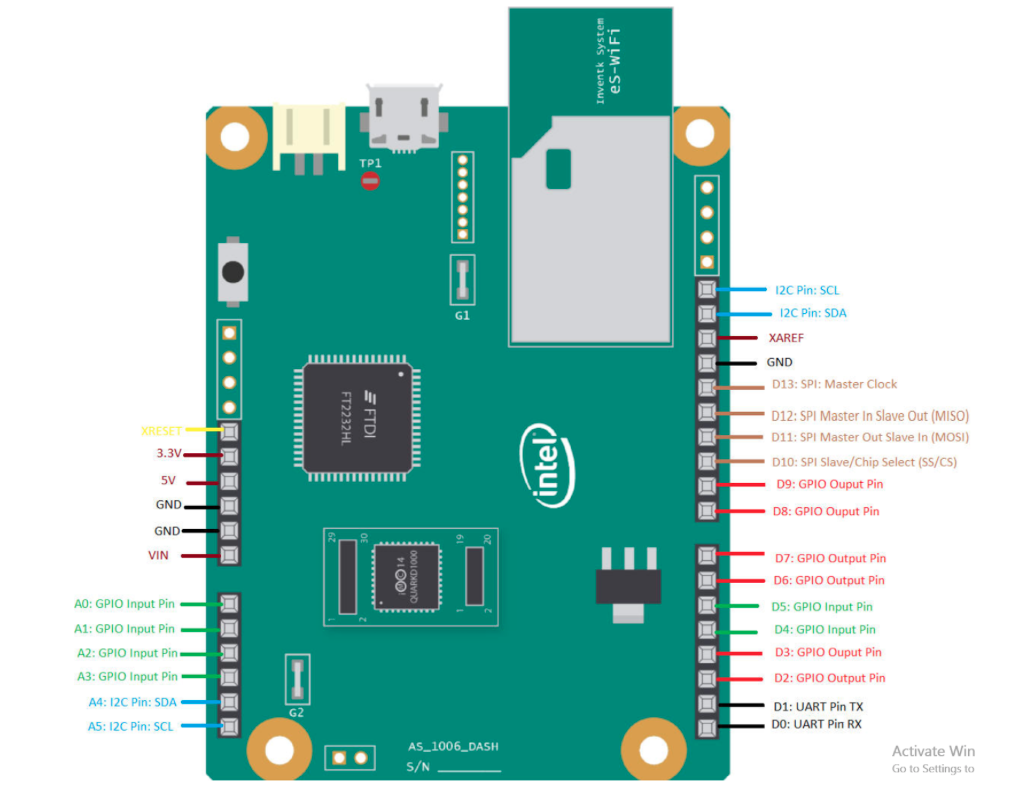
\includegraphics[width=14cm,height=0.7\textheight,keepaspectratio]{./figures/figure_9}
	\center\caption[font=footnote]{Board Layout of Galileo Gen2 5}
\end{figure}

The Galileo Gen 2 distribution of Java ME supports the GPIOPin classes, which allows for general purpose pin configuration and I/O, as well as I2C and others. Since the flame sensor uses digital signal (on or off) to alert of any flames detected  simply using the GPIOPin class to read the data sufficed.  It's important to note that while the standard distribution for Java ME (used in IDE's and emulators during development) does support the ADC( analog to digital conversion) classes, the distribution for Galileo Gen 2 does not. This meant reading from the pin would be significantly harder to do with Java. By nature, the ADC pins, as well as others, output data into a file that can be accessed through the command line, for example the output of the A0 pin could be read by looking at:  /sys/bus/iio/devices/iio:device0/in\_voltage0\_raw. Although Java has the ability to read from files, Java ME's JRE has different root directories making it more difficult to track down the proper file paths. The easiest way was to set up a symlink from the output file of the sensor to a file in Java ME JRE's root directory. Once the symlink was set up it was easy to set the correct file read permissions in the Application descriptor to allow for reading the data, rather than adding another permission related to ADC or GPIO pins.

Once the ability to gather information from the temperature and flame sensors had been established the data needed to be transmitted to the user. To accomplish this, client/server and message classes were created to facilitate data transfer. A mock up protocol was also created in order to transfer vital data that wasn't required to be encrypted, such as message lengths, key lengths, types of messages, and encryption schemes being used.  Without a mockup protocol it would be difficult for server/client to agree on encryption schemes(i.e. GCM vs AES). One should note, this protocol should not be used for real world applications and was simply created for testing the case study. Much of the case study was designed to be run using 128 bit symmetric keys and the curve secp128r1 for key generation and may work differently if other curves or key sizes are used.

We created server, client, and message classes to better organize the cast study and send data between a central node and the Fire Detection System. The central node (in this case a Macbook Pro was used)  would run the server class awaiting connection from the client (Fire Detection System). The classes support four types of messages. First, if a key exchange has not taken place and a symmetric key is not yet established between the two parties the client will send it's public key to the server. The server will respond by sending its public key and both parties will compute a shared secret which will then be derived into a symmetric key. 

Additional communication can take place using either no encryption, AES encryption with an HMAC for authentication and integrity, or AES/GCM which will also provided encryption, authentication and message integrity. Below are the findings. 


 \begin{table}[t]
	\centering
	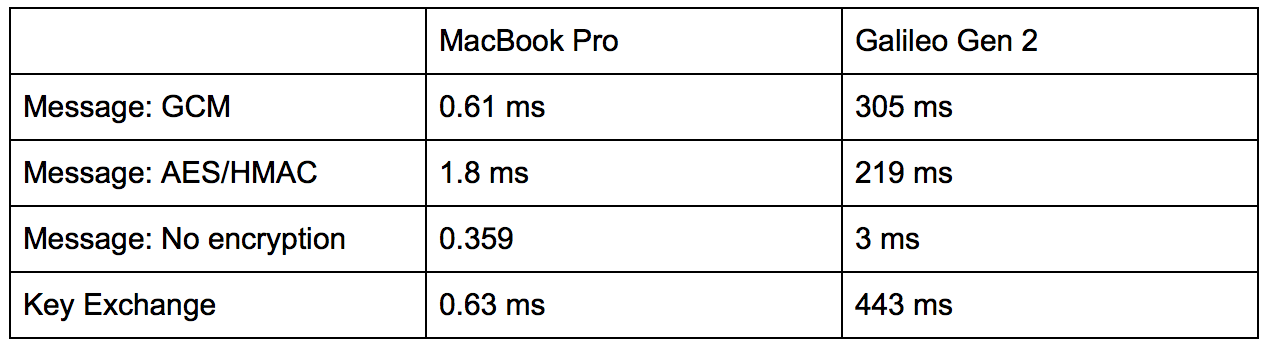
\includegraphics[width=11cm,height=0.7\textheight,keepaspectratio]{./figures/table_4}
	\center\caption[font=footnote]{Case Study Results}
\end{table}

Comparing these numbers to the results found in the previous section Results and Analysis, it is clear that there is a significant amount of overhead added with the protocol and network usage. In both cases for the Mac and Galileo the key exchange did not include key generation as it is assumed a key has already been generated. It is particularly strange that the Galileo took significantly longer to send a key but this may be due simply to the payload size. The biggest surprise is how fast using no encryption is compared to using either GCM or AES/HMAC. While encryption adds overhead, looking at the previously stated results made it seem like the overheard wouldn't be this significant. 

In an application like this it may be viable to deal with the overhead from encryption, authentication, and integrity. However, more vital, lower resource devices may suffer greatly from the implementation of these functions if the device is required to talk over a network frequently. 

\subsection{Implementation Issues}
There were a number of unanticipated issues that delayed the final product by up to a month. Many of these issues related back directly to Oracle's distribution of the Java ME platform where fixes or workarounds were few and far between. The first, and perhaps greatest, issue was related to Oracle's Java ME SDK distribution. In order to develop Java applications for embedded devices through Java ME, you are required to download and install a number of tools, namely the Java ME SDK. This SDK contains a number of useful and required tools for development, including a device manager and embedded emulators. The SDK is only distributed for Windows and has plugins for only  two IDEs: NetBeans and Eclipse.

 After installing both the SDK and the plugins for Eclipse you can create a Java ME project and are required to choose a embedded emulator configuration profile to test your application. A number of emulators are provided by the SDK and are managed by the device manager. However, contrary to the functionally outlined in the documentation, the IDE didn't recognize any of the emulator profiles and therefore would not allow for the creation of a Java ME project. After a number of days searching for a fix turned up nothing and trying different versions of both IDEs and the SDK with no success, an alternative workaround was sought. According to Oracle's documentation Java ME supported a subset of the libraries found in Java SE so it seemed logical to develop using only this subset of libraries in the Java SE environment. This turned out to be an unwise decision because, in fact, the libraries themselves contained a subset of the required classes and many of the classes had been reworked for Java ME.
 
 In short, a project developed in Java SE would not run in the Java ME environment. Looking back this seemed obvious, but at the time the list of options seemed short. Much of the developed code would have to be reworked and rewritten to run on Java ME which presented a set back, not only because much of the code was useless but also because Java ME's subset of the Java's Security library was missing a number of classes that were vital to the project. Luckily, Bouncy Castle, a well known distributor of open source security libraries, had a deployment of their security API specifically for Java ME. 
 
At this point, since the Java ME wasn't working with Eclipse or Netbeans, the project was developed in Intellij. However, this proved to be a source of its own issues since, while Intellij could run Java using the Java ME runtime environment, the IDE failed to build JAR files properly and consistently produced corrupt JAR files. Building the JAR files from the command line also failed to produce working outputs. At this point it seemed wise to return to trying to get the Java ME SDK to work properly. After reinstalling all the proper tools and scouring for answers, a fix was found. There was a recent post indicating a problem with the device manager provided by the Java ME SDK. During deployment a configuration file buried deep in the Java directory path was missing a number of lines that were vital to the operation of the device manager. Additionally the device manager was required for Java ME SDK to work at all, since almost the entire project, from the configuration files to the libraries used in the distribution, were all based on the configuration of the emulators. As expected, appending the missing lines to the configuration file caused the device manager to run properly. After more research, it was apparent that this bug had been cataloged but no official fix had been released and would not be released until Java ME 9.  

Documentation for the Intel Galileo Gen 2  and Java ME were also lacking in general, and documentation specific to Java ME was very hard to find or decipher. For example, figuring out how to set permissions for a Java ME project, or what Java libraries are actually supported in this particular distribution were not made obvious. In particular the documentation that related the Galileo to the Java ME distribution was difficult to find. While in part this is partially the fault of Oracle, there is almost no documented cases of other projects developed on the Galileo using Java ME. Clearly, Oracle has intended Java ME's use on the Galileo since they have a specific distribution for it, but either few people have used it or they ran into far fewer issues than we did on this project. 
